\section{InsertionSort}

\subsection{Algemeen}

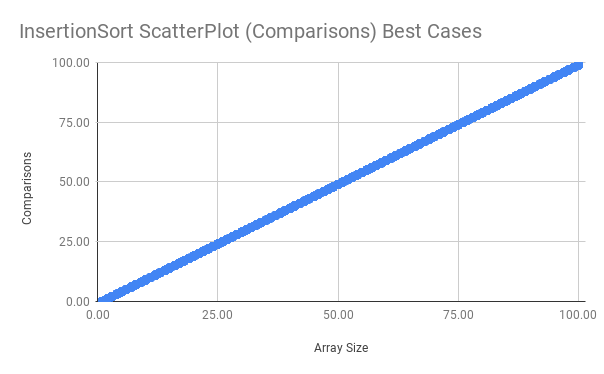
\includegraphics[scale=0.3]{sections/media/IS_C_BC}
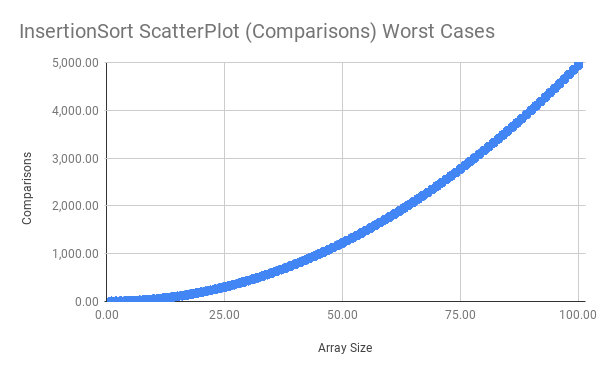
\includegraphics[scale=0.3]{sections/media/IS_C_WC}
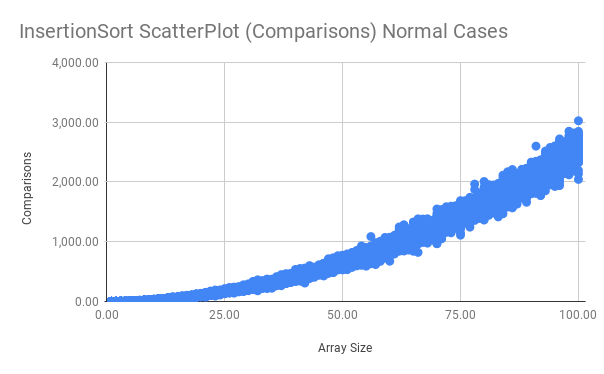
\includegraphics[scale=0.6]{sections/media/IS_C_NC}

InsertionSort is een sorteeralgoritme dat het definitief gesorteerde array een item tegelijk opbouwd. Theoretisch is InsertionSort een \(\sim n^{2}/4\) algoritme.

We kunnen zien dat in normale gevallen het algoritme afhanklijk is van de data in de array, en dat het sterk op een kwadratische functie lijkt.

Herkenbaar is ook dat het algoritme in het beste geval \(n\) vergelijkingen gaat maken, en dat in het slechste geval \((n^2 - n)/2\) vergelijkingen gaat maken.

\subsection{Doubling Ratio}
\begin{table}[hp!]
    \centering
    \begin{tabular} {c | c | c}
        \textbf{AS(N)} & \textbf{MT(N)} & \textbf{MR(N)} \\
        \hline
        640 & 0.85 ms & 1.70 \\
        \hline
        1 280 & 1.15 ms & 1.35 \\
        \hline
        2 560 & 4.70 ms & 4.09 \\
        \hline
        5 120 & 18.45 ms & 3.93 \\
        \hline
        10 240 & 74.65 ms & 4.05 \\
        \hline
        20 480 & 328.65 ms & 4.40 \\
    \end{tabular}
    \caption{InsertionSort Doubling Ratio Measurements}
\end{table}


Het doubling ratio experiment voor InsertionSort levert de bovenstaande tabel op. We verwachten dat het doubling ratio 4 nadert, want \(T(2)=2^2=4\). We zien ook dat de gemeten doubling ratio 4 nadert.

\begin{table}[hp!]
    \centering
    \begin{tabular} {c | c | c | c | c}
        \textbf{AS(N)} & \textbf{PT(N)} & \textbf{PR(N)} & \textbf{MT(N)} & \textbf{MR(N)} \\
        \hline 
        40 960 & 1 314.60 ms & 4.00 & 2 162.25 ms & 6.58 \\
        \hline
        81 920 & 5 258.40 ms & 4.00 & 8 426.65 ms & 3.90 \\
        \hline
        163 840 & 21 033.60 ms & 4.00 & 40 994.95 ms & 4.86 \\
    \end{tabular}
    \caption{InsertionSort Doubling Ratio Predictions}
\end{table}


Voor de voorspelling is het doubling ratio 4 gebruikt zoals hierboven uitgelegt.We zien uit de tabel dat de voorspelling ongeveer correct is. Als we nu een voorspelling maken voor een problem size N die 8 keer groter is dan onze grootste meting, volgt dat: \(40994.95*4^8=2686645043.2\) of 1 maand 16 uur 12 minuten en 37 seconden.
